\let\negmedspace\undefined
\let\negthickspace\undefined
\documentclass[journal,12pt,onecolumn]{IEEEtran}
\usepackage{cite}
\usepackage{amsmath,amssymb,amsfonts,amsthm}
\usepackage{algorithmic}
\usepackage{graphicx}
\usepackage{textcomp}
\usepackage{xcolor}
\usepackage{txfonts}
\usepackage{listings}
\usepackage{enumitem}
\usepackage{mathtools}
\usepackage{gensymb}
\usepackage[breaklinks=true]{hyperref}
\usepackage{tkz-euclide} % loads  TikZ and tkz-base
\usepackage{listings}



\newtheorem{theorem}{Theorem}[section]
\newtheorem{problem}{Problem}
\newtheorem{proposition}{Proposition}[section]
\newtheorem{lemma}{Lemma}[section]
\newtheorem{corollary}[theorem]{Corollary}
\newtheorem{example}{Example}[section]
\newtheorem{definition}[problem]{Definition}
%\newtheorem{thm}{Theorem}[section] 
%\newtheorem{defn}[thm]{Definition}
%\newtheorem{algorithm}{Algorithm}[section]
%\newtheorem{cor}{Corollary}
\newcommand{\BEQA}{\begin{eqnarray}}
\newcommand{\EEQA}{\end{eqnarray}}
\newcommand{\define}{\stackrel{\triangle}{=}}
\theoremstyle{remark}
\newtheorem{rem}{Remark}
%\bibliographystyle{ieeetr}
\begin{document}
%
\providecommand{\pr}[1]{\ensuremath{\Pr\left(#1\right)}}
\providecommand{\prt}[2]{\ensuremath{p_{#1}^{\left(#2\right)} }}        % own macro for this question
\providecommand{\qfunc}[1]{\ensuremath{Q\left(#1\right)}}
\providecommand{\sbrak}[1]{\ensuremath{{}\left[#1\right]}}
\providecommand{\lsbrak}[1]{\ensuremath{{}\left[#1\right.}}
\providecommand{\rsbrak}[1]{\ensuremath{{}\left.#1\right]}}
\providecommand{\brak}[1]{\ensuremath{\left(#1\right)}}
\providecommand{\lbrak}[1]{\ensuremath{\left(#1\right.}}
\providecommand{\rbrak}[1]{\ensuremath{\left.#1\right)}}
\providecommand{\cbrak}[1]{\ensuremath{\left\{#1\right\}}}
\providecommand{\lcbrak}[1]{\ensuremath{\left\{#1\right.}}
\providecommand{\rcbrak}[1]{\ensuremath{\left.#1\right\}}}
\newcommand{\sgn}{\mathop{\mathrm{sgn}}}
\providecommand{\abs}[1]{\left\vert#1\right\vert}
\providecommand{\res}[1]{\Res\displaylimits_{#1}} 
\providecommand{\norm}[1]{\left\lVert#1\right\rVert}
%\providecommand{\norm}[1]{\lVert#1\rVert}
\providecommand{\mtx}[1]{\mathbf{#1}}
\providecommand{\mean}[1]{E\left[ #1 \right]}
\providecommand{\cond}[2]{#1\middle|#2}
\providecommand{\fourier}{\overset{\mathcal{F}}{ \rightleftharpoons}}
\newenvironment{amatrix}[1]{%
  \left(\begin{array}{@{}*{#1}{c}|c@{}}
}{%
  \end{array}\right)
}
%\providecommand{\hilbert}{\overset{\mathcal{H}}{ \rightleftharpoons}}
%\providecommand{\system}{\overset{\mathcal{H}}{ \longleftrightarrow}}
	%\newcommand{\solution}[2]{\textbf{Solution:}{#1}}
\newcommand{\solution}{\noindent \textbf{Solution: }}
\newcommand{\cosec}{\,\text{cosec}\,}
\providecommand{\dec}[2]{\ensuremath{\overset{#1}{\underset{#2}{\gtrless}}}}
\newcommand{\myvec}[1]{\ensuremath{\begin{pmatrix}#1\end{pmatrix}}}
\newcommand{\mydet}[1]{\ensuremath{\begin{vmatrix}#1\end{vmatrix}}}
\newcommand{\myaugvec}[2]{\ensuremath{\begin{amatrix}{#1}#2\end{amatrix}}}
\providecommand{\rank}{\text{rank}}
\providecommand{\pr}[1]{\ensuremath{\Pr\left(#1\right)}}
\providecommand{\qfunc}[1]{\ensuremath{Q\left(#1\right)}}
	\newcommand*{\permcomb}[4][0mu]{{{}^{#3}\mkern#1#2_{#4}}}
\newcommand*{\perm}[1][-3mu]{\permcomb[#1]{P}}
\newcommand*{\comb}[1][-1mu]{\permcomb[#1]{C}}
\providecommand{\qfunc}[1]{\ensuremath{Q\left(#1\right)}}
\providecommand{\gauss}[2]{\mathcal{N}\ensuremath{\left(#1,#2\right)}}
\providecommand{\diff}[2]{\ensuremath{\frac{d{#1}}{d{#2}}}}
\providecommand{\myceil}[1]{\left \lceil #1 \right \rceil }
\newcommand\figref{Fig.~\ref}
\newcommand\tabref{Table~\ref}
\newcommand{\sinc}{\,\text{sinc}\,}
\newcommand{\rect}{\,\text{rect}\,}
%%
%	%\newcommand{\solution}[2]{\textbf{Solution:}{#1}}
%\newcommand{\solution}{\noindent \textbf{Solution: }}
%\newcommand{\cosec}{\,\text{cosec}\,}
%\numberwithin{equation}{section}
%\numberwithin{equation}{subsection}
%\numberwithin{problem}{section}
%\numberwithin{definition}{section}
%\makeatletter
%\@addtoreset{figure}{problem}
%\makeatother

%\let\StandardTheFigure\thefigure
\let\vec\mathbf


\bibliographystyle{IEEEtran}
\title{ GATE IN-13 2022}
\author{EE23BTECH11011- Batchu Ishitha$^{*}$% <-this % stops a space
}
\maketitle




\bigskip

\renewcommand{\thefigure}{\theenumi}
\renewcommand{\thetable}{\theenumi}
%\renewcommand{\theequation}{\theenumi}

Q: A periodic function $f(x)$, with period 2, is defined as \\
   \begin{align}   
   f(x) =
   \begin{cases}
    -1-x & -1 \leq x<0 \\
     1-x &  0 <x \leq1 
   \end{cases}
   \end{align} 
   The Fourier series of this function contains \\
\begin{enumerate}[label=\Alph*.]
\item Both $\cos(n\pi x)$ and $sin(n\pi x)$ where n=1,2,3...
\item Only $\sin(n\pi x)$ where n=1,2,3...
\item Only $\cos(n\pi x)$ where n=1,2,3...
\item Only $\cos(2n\pi x)$ where n=1,2,3...  \hfill{GATE IN 2022 }
\end{enumerate} 

\solution

\begin{table}[!ht]    
    \centering
    \begin{tabular}[12pt]{ |c| c|}
    \hline
    \textbf{Parameter} & \textbf{Description}\\ 
    \hline
    $f\brak{x}$ & Polynomial function\\
    \hline
    $2L$& Period of the Polynomial function\\ 
    \hline
    $c(n)$ & Complex Fourier Coefficients\\
    \hline
     \end{tabular}

    \caption{Input Parameters}
    \label{table:ishitha.g22.in.13.t1}
\end{table}

The complex exponential Fourier Series of $f\brak{x}$ is,
\begin{align}
    f\brak{x}&=\sum_{n=-\infty}^{\infty}c(n)e^{jn\omega x}\\
    \implies c(n)&=\frac{1}{2L}\int_{-L}^{L}f\brak{x}e^{-jn\omega x}\;dx\\
\end{align}    

For $n\neq 0$;
\begin{align}
c(n) &= \frac{1}{2} \int_{-1}^{1} f(x) e^{-jn\omega x} \, dx \\
&= \frac{1}{2} \brak{ \int_{-1}^{0}\brak{-1-x}e^{-jn\omega x} \, dx +  \int_{0}^{1}\brak{+1-x}e^{-jn\omega x} \, dx } \\
&= \frac{1}{2} \brak{-\int_{-1}^{0}e^{-jn\omega x} \, dx -\int_{-1}^{1}xe^{-jn\omega x} \, dx + \int_{0}^{1}e^{-jn\omega x} \, dx} \\
&= \frac{1}{2} \sbrak{\frac{-1}{jn\omega }\sbrak{-\brak{1 - e^{+jn\omega }} + \brak{e^{-jn\omega } -1}} -\int_{-1}^{1}xe^{-jn\omega x} \, dx} \\
&= \frac{1}{2} \sbrak{\frac{-1}{jn\omega }\sbrak{-2 +e^{+jn\omega } + e^{-jn\omega }} +\brak{\frac{e^{-jn\omega x}}{jn\omega }\sbrak{x + \frac{1}{jn\omega }}}_{-1}^{1}} \\
&= \frac{-1}{jn\omega }\sbrak{-1 + \cos(n\omega )} + \frac{1}{2(jn\omega )^2}\sbrak{\brak{e^{-jn\omega }}\brak{1+jn\omega }- \brak{e^{jn\omega } }\brak{-jn\omega +1}} \\
\implies c\brak{n}&= \frac{-1}{(jn\omega )^2}\sbrak{-jn\omega  + j \sin(n\omega )}
\end{align} 

For $n=0$;
\begin{align}
c(0) &= \frac{1}{2} \int_{-1}^{1} f(x) \, dx \\
&=  \frac{1}{2} \sbrak {\int_{-1}^{0} \brak{-1-x} \, dx + \int_{0}^{1} \brak{1-x} \, dx } \\
&= \frac{1}{2} \sbrak{ \brak{-x-\frac{x^2}{2}}_{-1}^{0} + \brak{x-\frac{x^2}{2}}_{0}^{1}} \\
&= \frac{1}{2} \sbrak{0-1+\frac{1}{2} +1 -\frac{1}{2} -0} \\
\implies c(0)&= 0
\end{align}


The trigonometric Fourier Series of $f\brak{x}$ is,
\begin{align}
    f\brak{x}=a(0)+\sum_{n=1}^{\infty}\cbrak{a(n)\cos\brak{n\omega x}+b(n)\sin\brak{n\omega x}}
\end{align}

Finding the Fourier Coefficient $a_0$,
\begin{align}
    a(0)&=c(0)\\
    \implies a(0)&= 0
\end{align}

Finding the Fourier Coefficients $a(n)$,
\begin{align}
    a(n)&=\frac{1}{L}\int_{-L}^{L}f(x)\cos\brak{n\omega x}\;dx, n \geq 0 \\
    &= \frac{1}{L}\int_{-L}^{L}f(x)\brak{e^{-jn\omega x}+e^{jn\omega x}} \; dx \\
 \implies a(n)   &= c(n) + c(-n) \\
 \implies a(n)&= 0 \\
\end{align}  
  
Finding the Fourier Coefficients $b(n)$,
\begin{align}
    b_n&=\frac{1}{L}\int_{-L}^{L}f(x)\sin\brak{n\omega x}\;dx, n \geq 0 \\
    &= \frac{1}{L}\int_{-L}^{L}f(x)j\brak{e^{-jn\omega x}-e^{jn\omega x}} \; dx \\
   \implies b(n) &= j\brak{c_{n} - c_{-n}} \\
   \implies b(n)&= \frac{-2}{(n\omega )^2}\sbrak{-n\omega +  \sin(n\omega)} 
\end{align}  

$\implies$ The trigonometric Fourier Series of $f\brak{x}$ is,
\begin{align}
 f\brak{x} &=\sum_{n=1}^{\infty}\cbrak{0+ 0 +b(n)\sin\brak{n\omega x}} \\
 f\brak{x} &=\sum_{n=1}^{\infty}\cbrak{\frac{-2}{(n\omega )^2}\sbrak{-n\omega +  \sin(n\omega)} \sin\brak{n\omega x}} \\
 f\brak{x} &=\sum_{n=1}^{\infty}\cbrak{\frac{-2}{(n\pi )^2}\sbrak{-n\pi +  \sin(n\pi)} \sin\brak{n\pi x}} \\
  f\brak{x} &=\sum_{n=1}^{\infty}\cbrak{\frac{2}{n\pi } \sin\brak{n\pi x}}
 \end{align}

 $\therefore$ The Fourier series of this function contains only $\sin(n\pi x)$ where n=1,2,3...
 
 \begin{figure}[!ht]
    \centering
     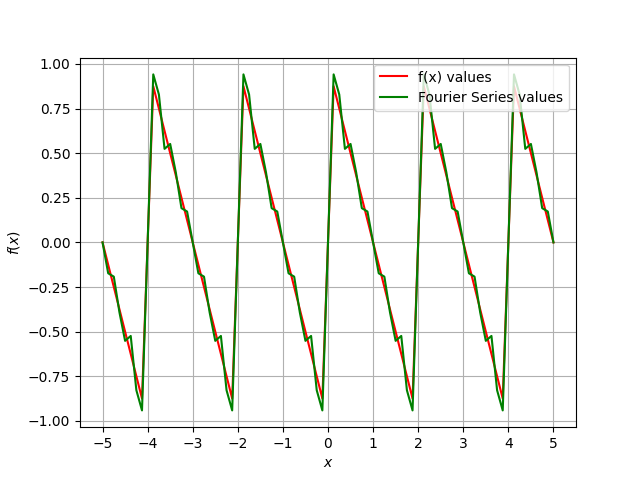
\includegraphics[width=\columnwidth]{./figs/f.png}
    \caption{}    
    \label{fig:ishitha.g22.in.13.f1}
\end{figure}
 

\end{document}
